\chapter{Performance Evaluation}
\label{Chapter5}
\lhead{Chapter 5. \emph{Performance Evaluation}} % Write in your own chapter title to set the page header

\section{Performance Metrics}
Life Span of the Network

Definition: The time when any node's battery die

Because the goal of this protocol is to broadcast any new packet, the network will lose the physical ability whenever any node lost wireless connection to its neighbors due to energy depletion. Therefore, this metric indicates how long a network with size n could stay connected using a broadcast protocol.

Average Packet Broadcast Time

Let's think about broadcasting one packet from one node to (n-1) nodes, the packet broadcast time of this packet for this network is the difference between the time when last node received the packet and the time this packet was first sent.

Because for each independent trial, multiple packets will be sent. The packet broadcast time is calculated for each packet in the way described above. In the end, we average the times for each scenario (e.g. n = 10). 

Need to develop a mathematical equation for this

The average packet broadcast time indicates the time needed for a packet to reach every node in the network.

Protocol Overhead

There are three types of protocol packets for the protocol. The ack packet, solicit packet, and the payload packet. The acknowledgment packet is sent to the sender from receiver when a node received a payload that it already received before. The solicit packet is sent to query a random neighbor for its latest payload. For example, in one trial with n nodes, if it broadcaster m packets, then the average protocol overhead is defined as:

$overhead = ()(p1 + p2 + … + p_n) / n) / m$

This metric indicated how many packets is needed for a node to facilitate broadcasting one packet. 

Consumed Energy

The consumed energy per node per packet is defined as

energy = ((e1 + e2 + … + en)/n)/m

This metric measures the amount of energy needed for a node to facilitate broadcasting one packet. 


\section{Simulation Data Process}
The simulation program output data files needs to be further processed in order to yield our performance metrics results. 

\begin{itemize}
	\item Average \msg ~broadcast time
	\item Average overhead
	\item Average energy consumption
	\item Network lifetime 
\end{itemize}

 

To evaluate the performance of gossip protocol, we use several randomly generated topology files with the number of nodes as variable. Those topology files are derived from a random geometric graph network, which was created by uniformly and randomly placing nodes into a space and then connect nodes whose distance is smaller than some given radius.



Each node holds an NS-3 Ipv4Interface with assigned Ipv4 address and stores the Ipv4 addresses of his neighbors.

For the simulation, we set the link rate for all connections to be 1Mbp. Also, all nodes are instructed to execute the gossip process of sending out data periodically every 5ms. The interval of requesting new data is set to 5s.

To allow the performance analysis, all nodes count the number of data packets they sent. All nodes would track how many hops the data message experienced before reaching them and they record the time when they received the data message as well. For every single simulation, we collect the information from the nodes and determine the average amount of data packets sent per node and average number of hops per node. Moreover, the information about how long it took for the message to reach the ``last'' node is also recorded.

This information is determined and stored for each of the several hundred topology files. It should be noted that due to time limitations each topology file was only simulated once. Finally, we did statistical analysis upon those collected data in the hope of verifying the assumptions we made in section~\ref{sec:problem}.

Talk about the settings


source DSSSRate 11Mbps
DsssRate 1Mbps
maxRange = 50m
num of nodes = 10
simulation time = 100000.0s
initialEnergy = 108J

Gossip Interval 1s
request interval 5s

In summary, the simulation parameters are set to be as follows:
\begin{itemize}
	\item Number of Nodes = 10, 20, 30, … , 200
	\item Simulation time = large enough to ensure energy depletion happens first
	\item Maximum Wifi Range = 50m
	\item Initial Energy = 108J
	\item Gossip Interval = 1.0s
	\item Solicit interval = 5.0s 
\end{itemize}

The number of nodes, simulation time, maximum wifi range, initial battery energy, gossip interval, and solicit interval are all the parameters I could control in the simulation. The number of nodes is ranging from 10 to 200 with step 10. The simulation time is set to be large enough to ensure any node's battery will die before the simulation stops. The maximum wifi range is set to be 50 meters so that no one node is connected to all other nodes. The initial battery energy is set to be 1080 Joule (equivalent to 100mAh) for every node. The gossip interval is set to be 1 second meaning for any node every second the gossip process will wake up and check if it need to gossip a new packet to its neighbors. The solicit interval is set to be 5 seconds which means every 5 seconds, a node will randomly pick a neighbor and query for their latest received packet. 




The simulation will stop when any node's energy was depleted. For each scenario (e.g. n = 10), 100 independent trials were simulated in order to gather performance data. Any simulation parameters other than number of nodes stay the same through all simulation trials. 


\section{Results Analysis}


\begin{figure}
	\centering
	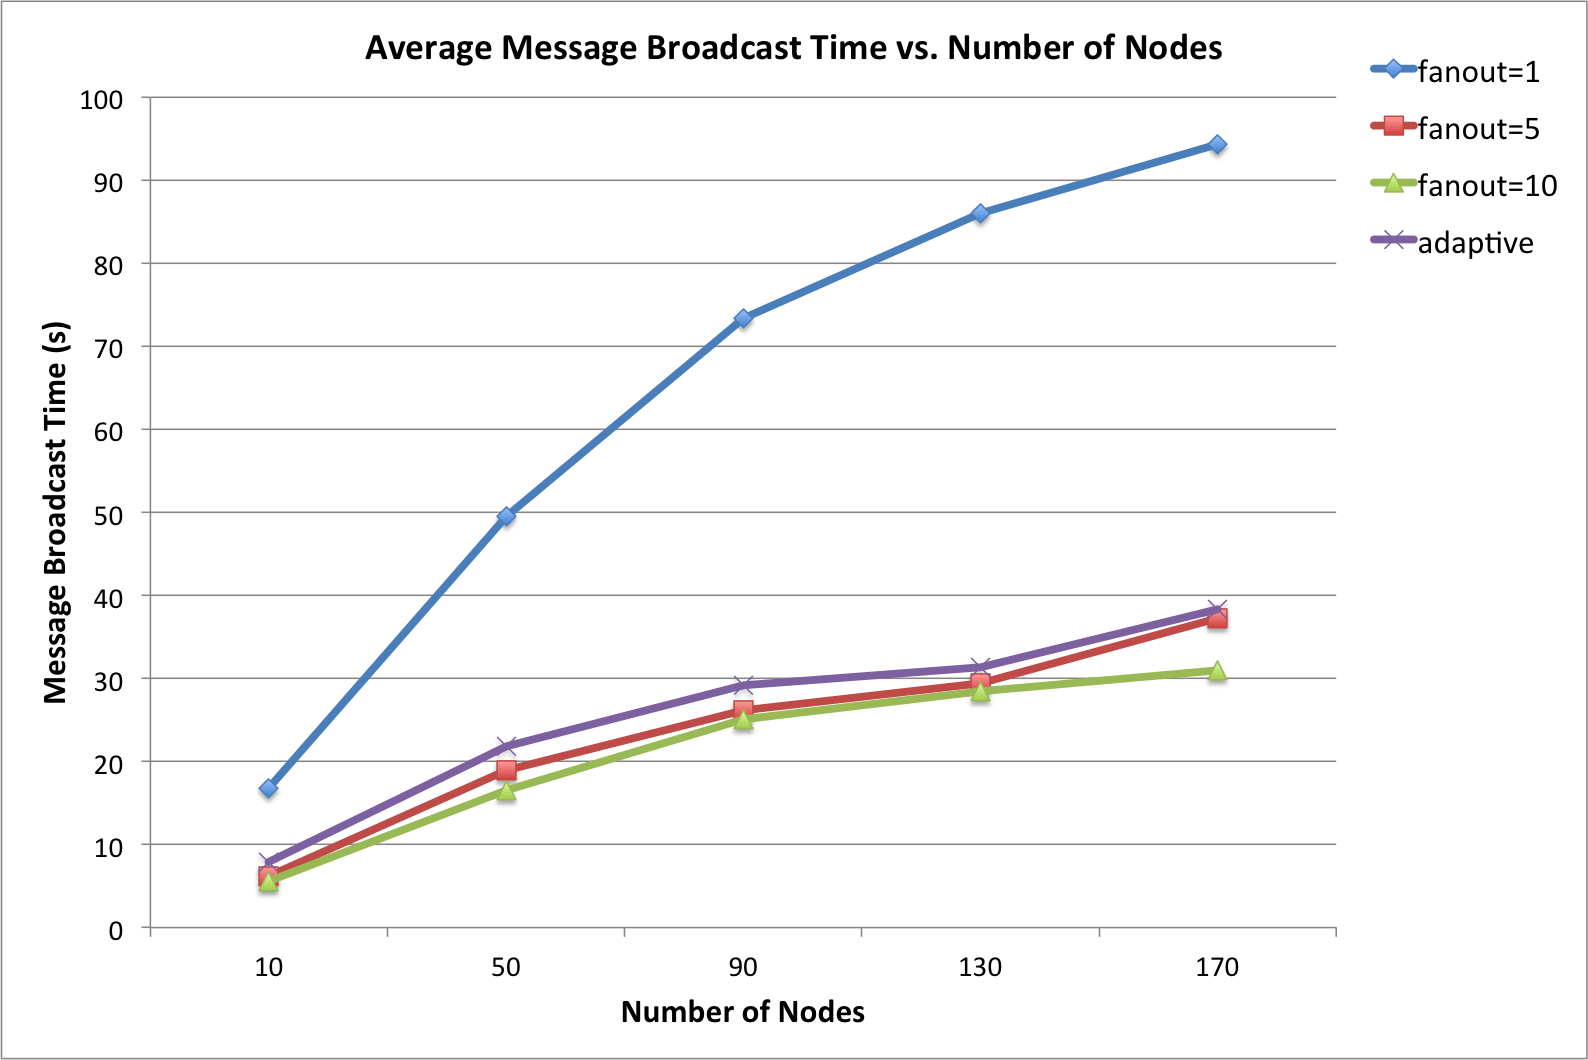
\includegraphics[width=3in]{brTime.png}
	\caption{Average message broadcast time vs. number of nodes}
	\label{fig:brTime}
\end{figure}

\begin{figure}
	\centering
	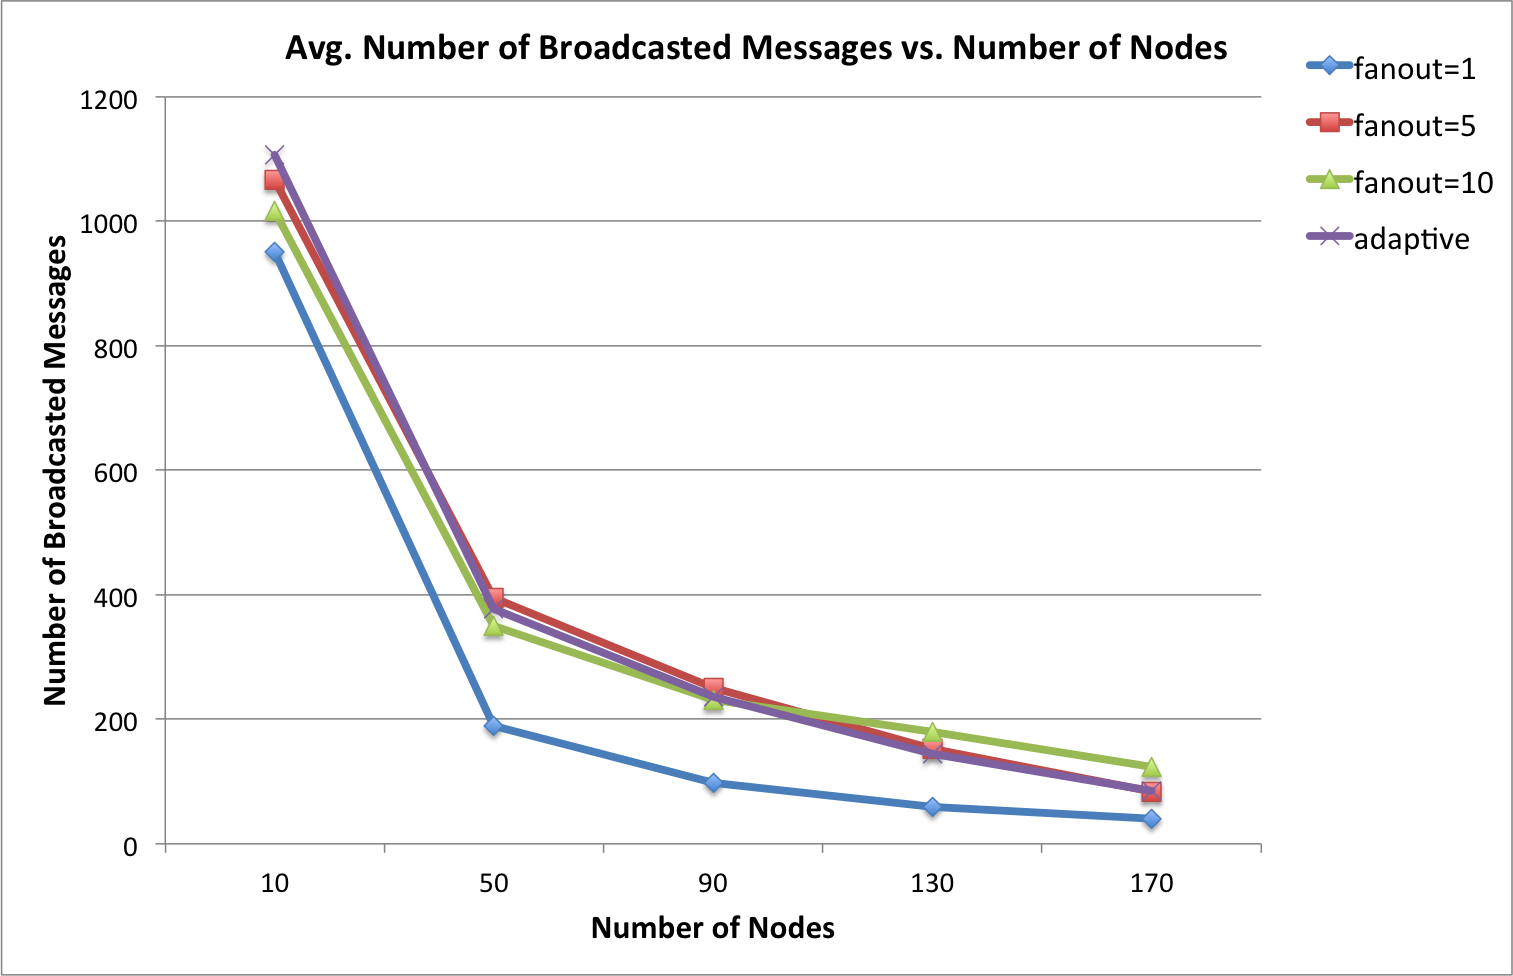
\includegraphics[width=3in]{brNum.png}
	\caption{Average number of broadcasted messages vs. number of nodes}
	\label{fig:brNum}
\end{figure}

\begin{figure}
	\centering
	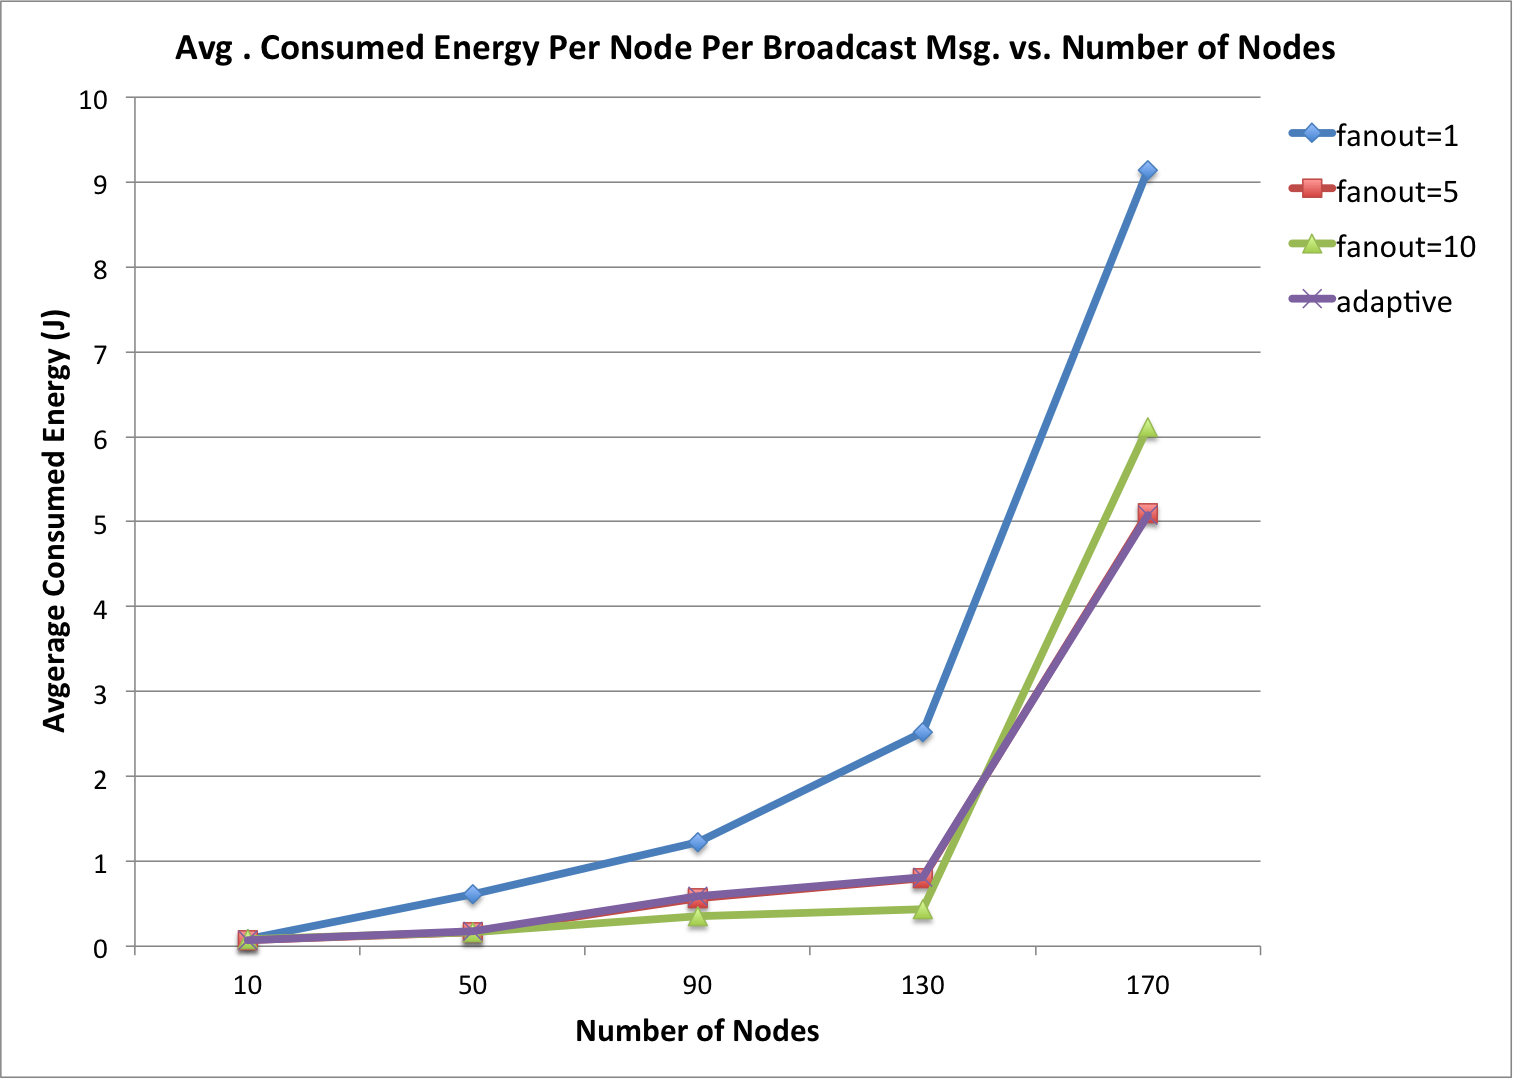
\includegraphics[width=3in]{energy.png}
	\caption{Average consumed energy per node per message vs. number of nodes}
	\label{fig:energy}
\end{figure}

\begin{figure}
	\centering
	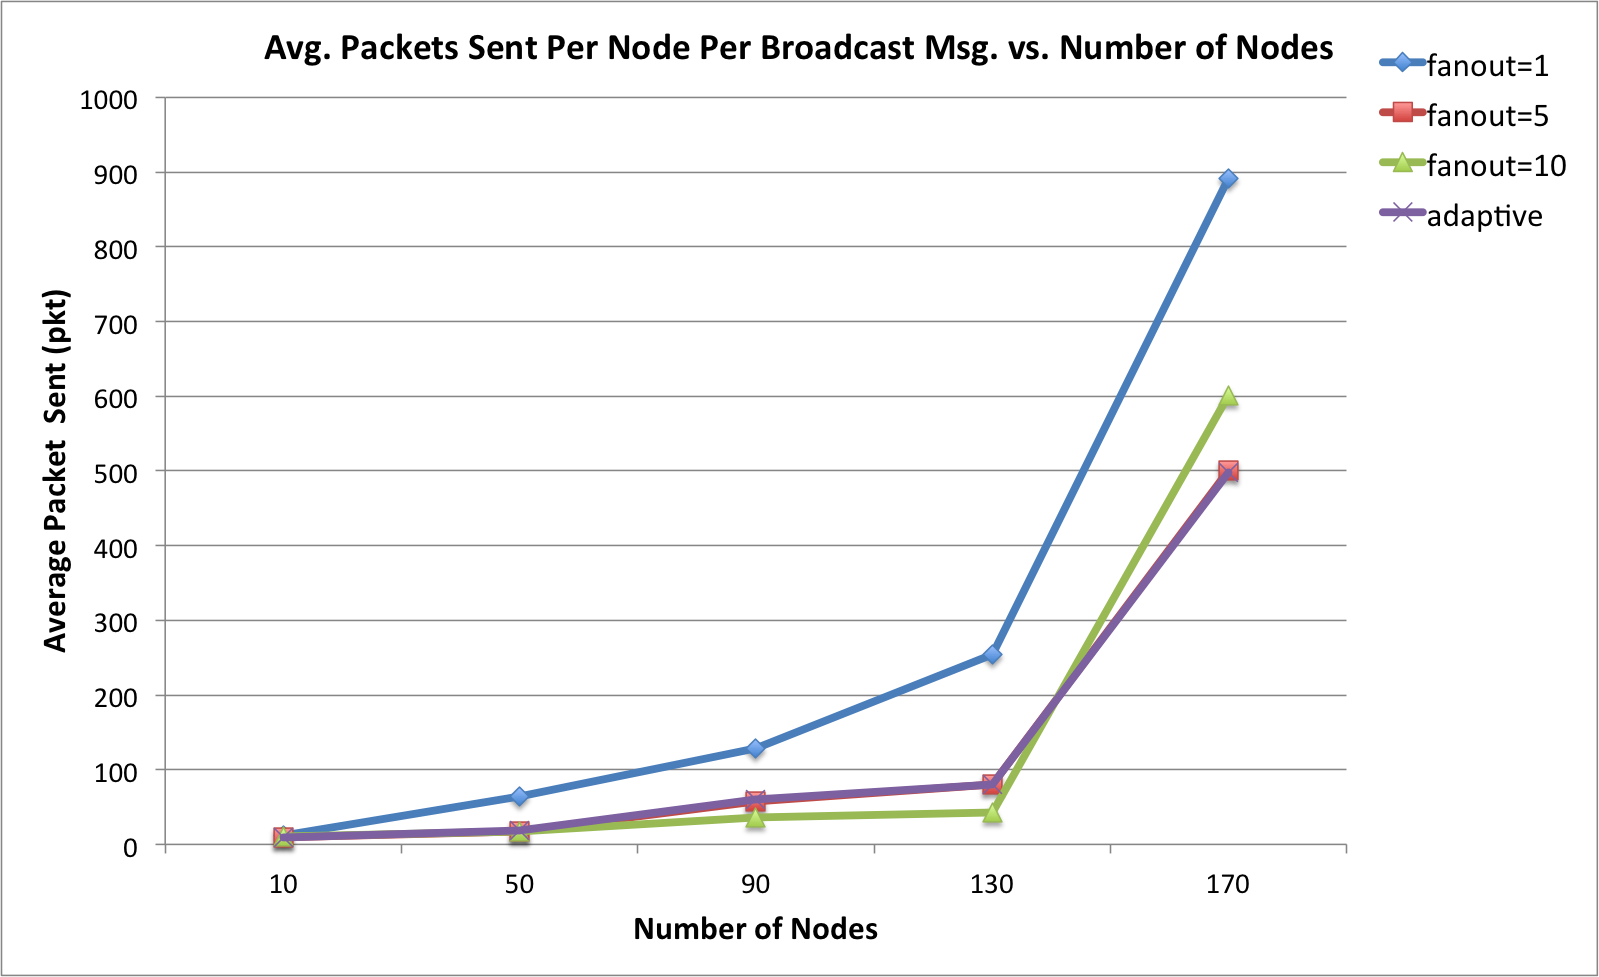
\includegraphics[width=3in]{overhead.png}
	\caption{Average packets sent per node per message vs. number of nodes}
	\label{fig:overhead}
\end{figure}

\begin{figure}
	\centering
	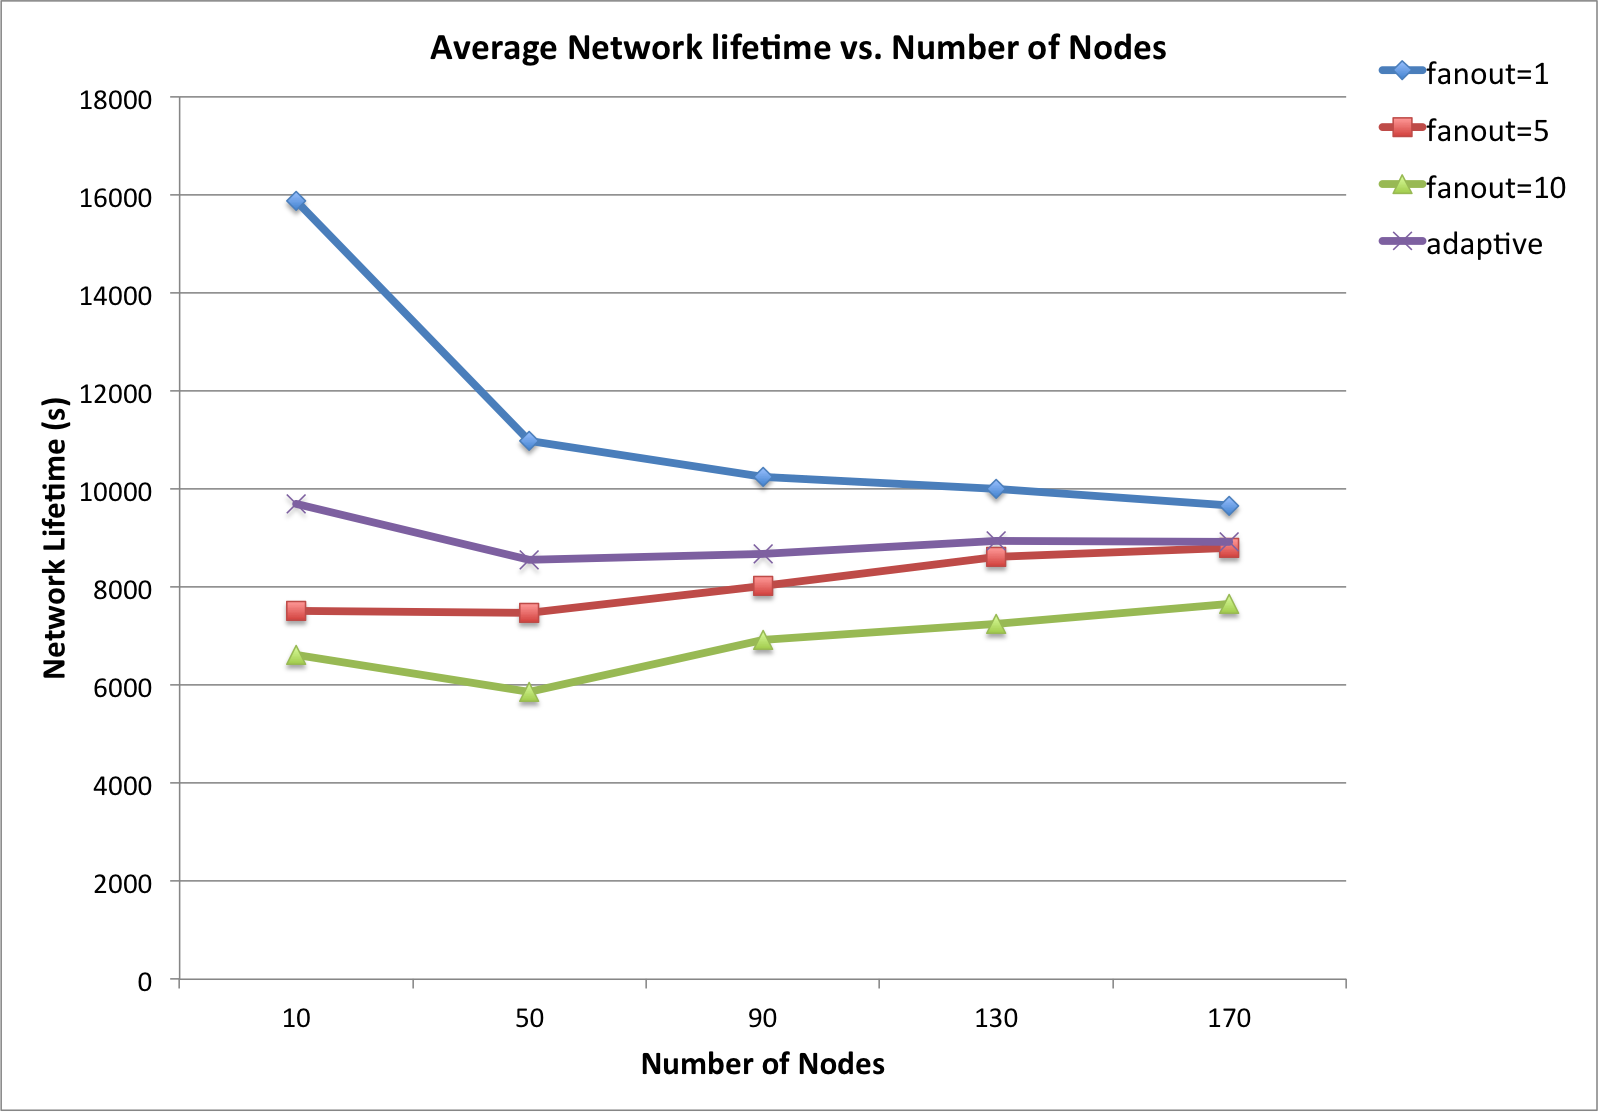
\includegraphics[width=3in]{life.png}
	\caption{Average network lifetime vs. number of nodes}
	\label{fig:life}
\end{figure}



Fanout of gossip protocol is defined as the number of neighbors a node contact each time when a new packet is received. It is one of the parameters that control the behavior of gossip protocol. In one scenario, fanout is set to be one. In another scenario, fanout is set to be five. These two scenarios 's trials are conducted to compare to the adaptive fanout scenario. 

(from 563 paper).

The random generated topology files are the input of our simulations. There are 7 different cases where the number of nodes vary from 100 to 1000 , increasing with 150 nodes step. And for each case, we sampled 100 topology files to run the simulations.

First, I analyzed the average number of data packets each node sent, depicted in fig.~\ref{fig:msgAbs}. It is important to note that the the collected average number for one topology file was again averaged over all reported values produced by topology files with the same number of nodes. Thus, the error bar is an indicator how consistent the average number is. It can be deduced from fig.~\ref{fig:msgAbs} that this value is ranging from 190 data packets per node to 280 data packets per node depending on the scale of the network. But considering the network scale, average number of data packets per node didn't increase proportionally as we can see in fig.~\ref{fig:msgOver}. This metrics actually decreased exponentially. 

%\begin{figure}
%	\centering
%	\includegraphics[width=3in]{figs/msgAbs}
%	\caption{The average number of data packets each node sent (Ad-hoc environment)}
%	\label{fig:msgAbs}
%\end{figure}
%
%\begin{figure}
%	\centering
%	\includegraphics[width=3in]{figs/msgOver}
%	\caption{The average number of data packets each node over the size of the network (Ad-hoc environment) }
%	\label{fig:msgOver}
%\end{figure}
%
%\begin{figure}
%	\centering
%	\includegraphics[width=3in]{figs/msgP}
%	\caption{The average number of ICMP messages each node sent (P2P environment)}
%	\label{fig:msgP}
%\end{figure}

Since when I collected the different data (average ICMP messages per node) from wired peer-to-peer network environment, here I could not perform a fair comparasion between these two evnironment. But as you can see in fig.~\ref{fig:msgP}, the average ICMP messages per node is significantly lower than in the wireless ad-hoc network. I believe the reason behind this is the shared medium for wireless communication. With shared medium, collision is prone to occur thus RTS/CTS plays an important role during the whole communicating process. Thus higher average data packets sent per node is expected.

Second, the average number of hops per node is analyzed. This is different from what we collected in the P2P environment which is maximum number of hops. Thus fair comparison between these two environment can not be performed here. In the wireless ad-hoc network, as we can see in fig. ~\ref{fig:hop}, the average number of hops per node mostly concentrated around 2.3 hops regardless of the growing number of nodes. For wired P2P network, the maximum hops is around 16.5. But the standard deviation has the tendency to decrease which is a positive sign since we hope the gossip protocol performance metrics would converge as the network grows. Nonetheless, the overall impression for both network environment is that the number of hops either average or maximum are more or less constant. But why is that the average hops per node could remaine 2 to 3 in a wireless ad-hoc network? My explaination is that since the topology of the network is almost a complete graph as you can see in fig.~\ref{fig:graph} showing a simple 10 nodes case, with gossip interval 5ms and request interval 5s, before any node send out request packets, chances are the starting node already gossipped with most of the node in the network result to a low average hops per node.

%\begin{figure}
%	\centering
%	\includegraphics[width=3in]{figs/hop}
%	\caption{The average number of hops per node (Ad-hoc environment).}
%	\label{fig:hop}
%\end{figure}
%
%\begin{figure}
%	\centering
%	\includegraphics[width=3in]{figs/hopP}
%	\caption{The maximum amount of hops the message experienced (P2P environment).}
%	\label{fig:hopP}
%\end{figure}
%
%\begin{figure}
%	\centering
%	\includegraphics[width=3in]{figs/Net_10}
%	\caption{A simple ten nodes random generated topology.}
%	\label{fig:graph}
%\end{figure}

Moreover, figure~\ref{fig:time} illustrates the time needed to spread the message across the whole network. For the P2P network environment, the average time needed to spread the message is found to be more or less constant and slightly less than 15s. Due to the huge difference in the gossip-interval-time (5ms) and solicit-interval-time (5s), only the influence of the solicit-interval can be deduced from the results. One can see, that the time needed to spread the message is fluctuating due to the random nature of the gossip protocol, especially for the case of a number of nodes of 100, where the standard deviation is the largest. However, when we compare this result with ad-hoc network simulation result, the different between them is significant. For the latter case, the spread time starts around 190s and grows almost linearly with the number of nodes in the network. In term of absolute maginitude, wireless network perform much worse than P2P network. However, this result is total within our expectation since wireless communication often encounter collision problem and thus result in longer spread time.

%\begin{figure}
%	\centering
%	\includegraphics[width=3in]{figs/time}
%	\caption{The spread time under different number of nodes cases}
%	\label{fig:time}
%\end{figure}

Section~\ref{sec:further} proposes further work which can be done to gain a more thorough evaluation.




